\documentclass{beamer}
\usepackage[utf8]{inputenc}
\usepackage[francais]{babel}
\usepackage[T1]{fontenc}

\usetheme{Madrid}
\usecolortheme{default}

\title[Algorithmique du Texte]{Algorithme de Aho-Corasick}
\author{E.Montagne, F.Van-Liedekerke}
\institute[]{Université de Rouen Normandie\\
UFR Sciences et Techniques
}

\begin{document}

  \frame{\titlepage}

  \begin{frame}
    \frametitle{Implémentation de l'algorithme d'Aho-Corasick}

    Pour implanter l'algorithme d'Aho-Corasick, nous allons avoir besoin de 
    plusieurs strucutres de données :
    \begin{itemize}
      \item Un trie
      \item Une file
      \item Une liste
    \end{itemize}

  \end{frame}

  \begin{frame}
    \frametitle{Présentation des deux implantations des tries}
    Deux manières de faire :
    \begin{itemize}
      \item Avec une matrice de transitions
      \item Avec une table de hacahge
    \end{itemize}
    
  \end{frame}

  \begin{frame}
    \frametitle{Matrice de transitions}
    
    Pourquoi utiliser une table de transitions?

  \end{frame}

  \begin{frame}
    \frametitle{Matrice de transitions}
    Avantages :
    \begin{itemize}
      \item Faible complexité en temps
      \item Facilité de mise en oeuvre
    \end{itemize}
    Incovénients :
    \begin{itemize}
      \item Complexité en espace élevée
    \end{itemize}
  \end{frame}

  \begin{frame}
    \frametitle{Table de hacahge}
    
    Pourquoi utiliser une table de hachage?

  \end{frame}

  \begin{frame}
    \frametitle{Table de hacahge}
    Avantages :
    \begin{itemize}
      \item Faible complexité en espace
    \end{itemize}
    Incovénients :
    \begin{itemize}
      \item Complexité en temps plus élevée qu'avec les matrices
    \end{itemize}
  \end{frame}

  \begin{frame}
    \frametitle{Quel trie choisir?}

    En fonction du nombre de mots il peut être judicieux de 
    choisir un trie plutôt qu'un autre.
    \newline
    \newline
    Nous verrons dans un second temps des graphiques qui nous 
    montrent la différence en temps de chacune des solutions.
  \end{frame}

  \begin{frame}
    \frametitle{File}

    Une fois notre trie créé, nous avons besoin de faire un parcours en largeur.
    D'où la nécessité d'avoir une file.
    \newline
    \newline
    Pour cela, nous avons implanté une file simple, avec des opérations pour
    insérer, et retirer des éléments de la file.

  \end{frame}

  \begin{frame}
    \frametitle{Liste}

    Nous avons aussi besoin de stocker des transitions, 
    d'où la nécessité d'implater aussi une liste
    \newline
    \newline
    Comme pour la file, nous avons implanté une liste simple, 
    avec des opérations pour insérer, et retirer des éléments de la liste.

  \end{frame}

  \begin{frame}
    \frametitle{Comparaison en temps des deux implantations de l'algorithme}
    \begin{center}
      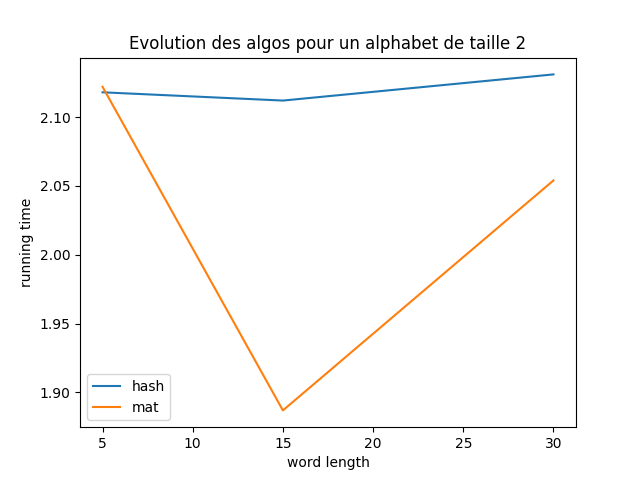
\includegraphics[scale = 0.5]{../Courbes/alphabet_2.png}
    \end{center}
  \end{frame}
  
  \begin{frame}
    \frametitle{Comparaison en temps des deux implantations de l'algorithme}
    \begin{center}
      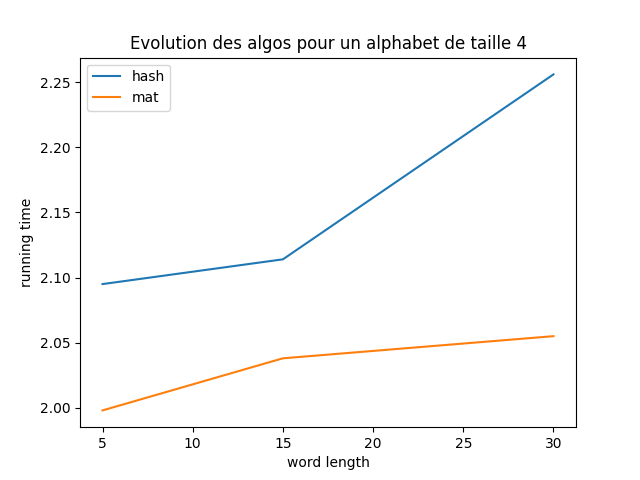
\includegraphics[scale = 0.5]{../Courbes/alphabet_4.png}
    \end{center}
  \end{frame}

  \begin{frame}
    \frametitle{Comparaison en temps des deux implantations de l'algorithme}
    \begin{center}
      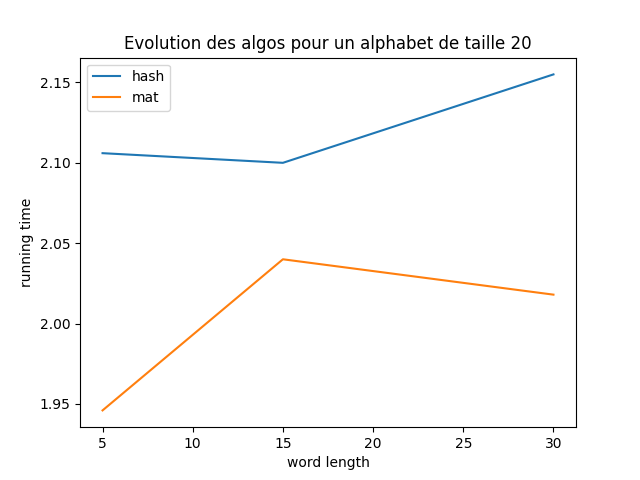
\includegraphics[scale = 0.5]{../Courbes/alphabet_20.png}
    \end{center}
  \end{frame}

  \begin{frame}
    \frametitle{Comparaison en temps des deux implantations de l'algorithme}
    \begin{center}
      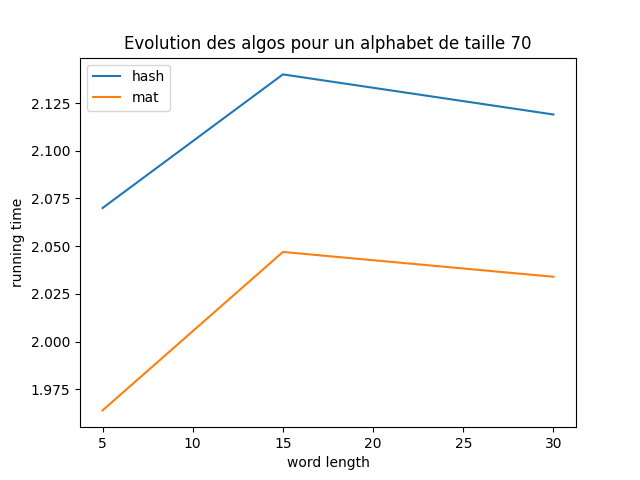
\includegraphics[scale = 0.5]{../Courbes/alphabet_70.png}
    \end{center}
  \end{frame}

  \begin{frame}
    \frametitle{Comparaison en temps des deux implantations de l'algorithme}
    \begin{center}
      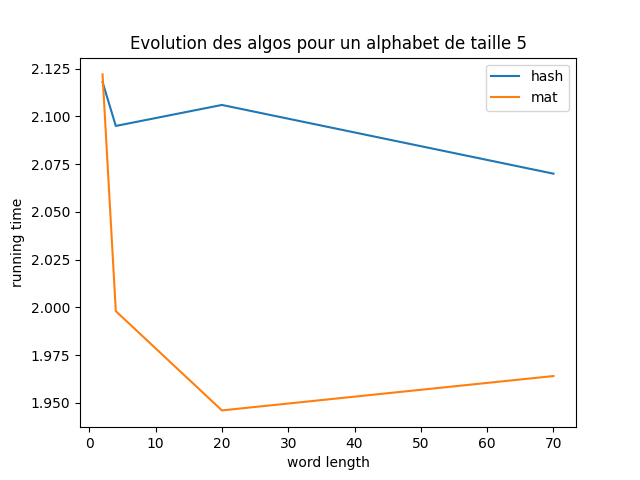
\includegraphics[scale = 0.5]{../Courbes/word_5.png}
    \end{center}
  \end{frame}

  \begin{frame}
    \frametitle{Comparaison en temps des deux implantations de l'algorithme}
    \begin{center}
      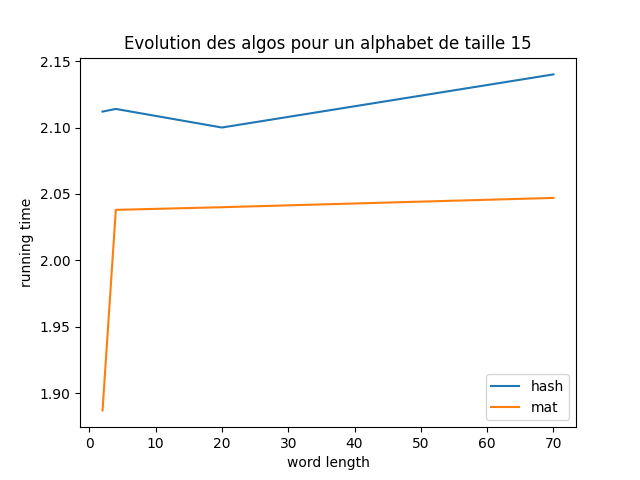
\includegraphics[scale = 0.5]{../Courbes/word_15.png}
    \end{center}
  \end{frame}

  \begin{frame}
    \frametitle{Comparaison en temps des deux implantations de l'algorithme}
    \begin{center}
      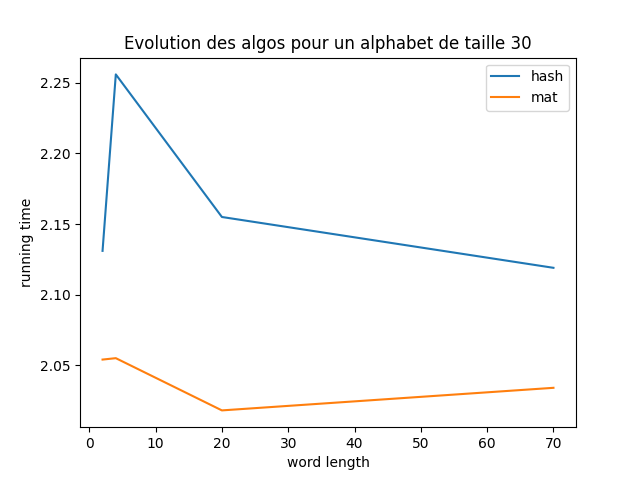
\includegraphics[scale = 0.5]{../Courbes/word_30.png}
    \end{center}
  \end{frame}

\end{document}